% compile using latex (xelatex seems to crop the figure strangley)
\documentclass{article} % For LaTeX2e
\usepackage[dvips]{graphicx}
\usepackage{nips14submit_e,times}
\usepackage{hyperref}
%\usepackage{wrapfig}
\usepackage{rotating}
\usepackage[outdir=./]{epstopdf}

\usepackage{graphics,graphicx}
\usepackage{amsmath,amssymb,amsfonts,comment}
\definecolor{LinkColor}{rgb}{0,0,0}    

\newcommand{\p}{\text{P}}
\newcommand{\word}[1]{\texttt{#1}}
\urldef{\googlegroup}\url{https://groups.google.com/forum/#!forum/word2vec-toolkit}
\urldef{\blogpost}\url{https://blog.lateral.io/2015/06/the-unknown-perils-of-mining-wikipedia/}

\title{Corpus Experiments for Word Embeddings}

 \author{
 	Benjamin Wilson\\
	Lateral GmbH\\
	\texttt{benjamin@lateral.io}
	\And
	Adriaan Schakel\\
	NNLP\\
	\texttt{adriaan.schakel@gmail.com}
 }

\date{\today}
\nipsfinalcopy % Uncomment for camera-ready version

\begin{document}

\graphicspath{{../outputs/}}
\maketitle


\begin{abstract}
	We introduce an experimental approach to studying the properties of word embeddings.
	Controlled experiments, acheived by modification of the training corpus, permit the demonstration of direct, causal relationships between word properties and word vector direction and length.
	This approach is demonstrated in the case of the word2vec CBOW model with experiments that independently vary word frequency and word co-occurrence noise.
	It is shown in this case that word vector length depends directly and essentially linearly on both word frequency and the level of noise in the co-occurrence distribution of the word.
	In both cases, the coefficient of linearity depends upon the word.
\end{abstract} 

\begin{section}{Introduction}
Word embeddings are typically trained with samples from the word co-occurrence distributions.
Recall that the co-occurrence distribution of a word $w$ gives the probability $\p(w'|w)$ that a word $w'$ occurs nearby, given that $w$ occurred.
Samples of the co-occurrence distributions are obtained by scanning a short window over the text.
The neighbouring words are treated as samples of the co-occurrence distribution the current word. 
Viewed in this way, the word vectors of the word embedding are determined by the co-occurrence distributions and frequencies of the words in the corpus.

In this short note, we perform experiments that illustrate the effect of these two determining pieces of information (the co-occurrence distribution and the word frequency) as they are varied independently of one another.
This is acheived through the introduction of new tokens into the training corpus with varying frequencies and varying levels of noise in their co-occurrence distributions.
The frequency and co-occurrence distributions of these introduced tokens are modelled on existing words in the corpus.

We illustrate our approach in case of the word2vec CBOW model.
However, these experiments (and other besides) could might equally well be performed for word embedding methods such as word2vec skip-gram \cite{DistRepns,EfficientEstimation}, GloVe \cite{pennington2014glove} and SENNA \cite{collobert-2011}.

In the case of word2vec, we show that word vector length depends directly on both word-frequency and the level of noise in the co-occurrence distribution of the word in an essentially linear manner.
In both cases, the coefficient of linearity depends upon the word.
If the co-occurrence distribution is fixed, then word vector length decreases with increasing word frequency.
On the other hand, if word frequency is held constant, then word vector length decreases as the level of  noise in the co-occurrence distribution of the word is increased.

We show furthermore that word vector direction does not vary with word frequency or with the level of co-occurrence noise.

This short note is structured as follows.
Section \ref{related-work} draws connections to related work, while Section \ref{corpus-and-model} describes the corpus and model used to illustrate the experiments.
Section \ref{WFVE} describes controlled experiment for varying word frequency while holding the co-occurrence distribution fixed.
Section \ref{CNVE}, in a complementary fashion, describes a controlled experiment for varying the level of noise in the cooccurrence distribution of a word, while holding the word frequency fixed.
Section \ref{future-directions} considers further questions and possible future directions.
\end{section}

\begin{section}{Related work}\label{related-work}
Our experimental finding (in the context of word2vec), that word vector length decreases with co-occurrence noise is reminiscent of \cite{vecchi-baroni-zamparelli2011}, where a relationship between vector length and the ``semantic deviance'' of an adjective-noun composition was studied observationally.
In \cite{schakel-wilson}, the interpretation of word vector length as an indication of word significance is explored in the context of the arXiv high-energy physics corpus.

\textcolor{red}{what about some work introducing tokens into a corpus for experiments?}

In the word2vec similarity and word relationship tasks, normalised word vectors are used.
Word vector length is thus disregarded.
In the word2vec forum\footnote{\googlegroup}, it has been observed that normalisation improves performance on these tasks since word vector length is related to word frequency.
Figure \ref{fig:frequency-norm-graph} illustrates the global relationship between vector length and word frequency.
It remained unclear, however, whether word frequency was \textit{directly} related to word vector length or rather via correlated factors such as word significance.
Our experimental approach demonstrates that a direct relationship indeed exists.
It is shown moreover that the normalisation of the word vectors also prevents word co-occurrence noise from affecting the performance of the word similarity and word relationship tasks.

On the other hand, recent theoretical work \cite{Arora2015} has approached the problem of explaining the so-called ``compositionality'' property exhibited by some word embeddings and that has been the subject of much recent attention.
In that work, unnormalised vectors are used in their model of the word relationship task.
It is hoped that experimental approaches such as those described here might yield insights into the role of the word vector length in the word relationship tasks.
\end{section}

\begin{section}{Corpus and model}\label{corpus-and-model}
Our training data is built from the Wikipedia XML datadump from October 2013.
In order to remove from the training data the bulk of robot-generated pages on Wikipedia, only pages with at least 20 monthly page views are retained\footnote{For further justification of this rationale, and to obtain the dataset, see \blogpost}.
Stubs and disambiguation pages are also removed, leaving 463 thousand pages with a total of 482 million words.

This base corpus is then modified as described in sections \ref{WFVE} and \ref{CNVE}.
Punctuation and numbers were removed and the corpus lower-cased prior to the modifications.
For recognisability, the tokens introduced into the corpus during the modification are uppercased.

For simplicity, only the word2vec CBOW word embedding with a single set of hyperparameters is considered.
Specifically, a $100$-dimensional CBOW model is trained using negative sampling with 5 negative samples, a window size of $10$, a minimum word occurrence of $128$, and $10$ passes through the corpus.
Subsampling was not used so that the influence of word frequency could be more clearly discerned.
Identical experimental results were obtained using hierarchical softmax, but these are omitted for succinctness.
The relatively high minimum word cut-off is chosen to ensure that word vectors receive a sufficient number of gradient updates to be meaningful.
\textcolor{red}{This cut-off results in a vocabulary of $62025$ words (only unigrams were considered).}

The most recent revision of word2vec was used\footnote{SVN revision 42, see \url{http://word2vec.googlecode.com/svn/trunk/}}.
The source code for performing the experiments is made available on GitHub\footnote{\url{https://github.com/benjaminwilson/word2vec-norm-experiments}}.

Word vectors are then derived from the first layer of synaptic weights (``syn0'') and the second layer of weights (``syn1neg'') are discarded.


\begin{figure}\label{fig:frequency-histogram}
	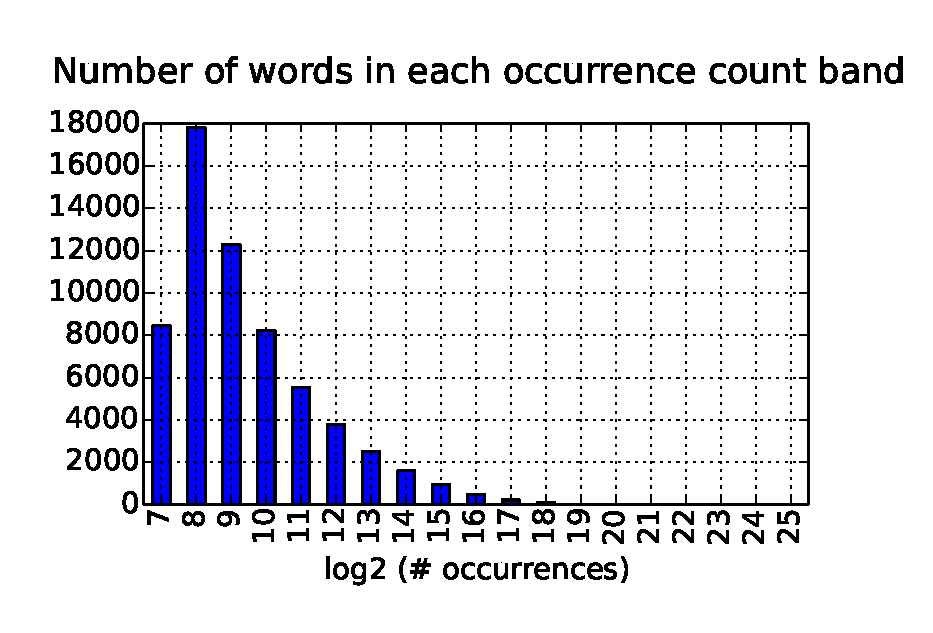
\includegraphics[scale=0.5]{occurrence-histogram}
	\caption{
	Number of vocabulary words by frequency band.
	}
\end{figure}

\begin{subsection}{Replacement procedure}\label{replacement-procedure}
In the experiments, tokens are introduced into corpus via a replacement procedure.
To illustrate this procedure, consider a word, e.g. \word{cat}.
For each occurrence of this word, a sample $i$, $1 \leqslant i \leqslant n$ is drawn from a truncated geometric distribution, and that occurrence of \word{cat} is replaced with \word{CAT\_i}.
Thus the word \word{cat} is replaced throughout the corpus by a family of tokens with varying frequencies but approximately the same co-occurrence distribution as \word{cat}.

The geometric distribution is truncated in order to limit the number of tokens introduced into the corpus.
For any ratio $0 < \lambda < 1$ and maximum value $n > 0$, the truncated geometric distribution is given by
$$ P_{\lambda, n} (i) = \frac{\lambda^{i-1} \cdot (1-\lambda)}{(1 - \lambda^n)}, \qquad 1 \leqslant i \leqslant n.$$ 
This is the distribution over $i = 1, 2, \dots n$ for which the probabilities decay exponentially base $\lambda$.
Of course, other distributions might equally have been chosen for the experiments.
\end{subsection}
\end{section}

\begin{section}{Word frequency variation experiment}\label{WFVE}
In this experiment, families of tokens are introduced into the corpus.
The tokens in each family vary in frequency but share a common co-occurrence distribution.
After model training, comparison of the resulting word vectors associated to these tokens reveals the independent effect of frequency variation on the word embedding.

\begin{subsection}{Tokens derived from existing words}\label{WFVEexisting}
A small set of words from the unmodified corpus is chosen uniformly at random from the vocabulary.
In order that the introduced tokens do not have too low a frequency, only words which occur at least 10 thousand times are chosen.
To this set of words, the word \word{the} is added, in order to include a high-frequency stopword.
The replacement procedure of subsection \ref{replacement-procedure} is then performed for each of these words, using a geometric rate of decay of $\lambda = 1/2$, and maximum value $n=20$.
This value of $\lambda$ is one of a range of values that ensure that, for each word, multiple tokens will be introduced with a number of occurrences sufficient to survive the chosen word2vec minimum occurrence cut-off of 128.  
A maximum value $n=20$ suffices for this choice of $\lambda$, since $2^{20 + \log_2{128}}$ exceeds the maximum occurrence of any token in the corpus. 
Figure \ref{fig:word-frequency-experiment-text-cat} illustrates the effect of these modifications on a sample text, with a family of tokens \word{CAT\_i}, derived from the word \word{cat}.
Notice that the word \word{cat} has been replaced throughout with the tokens \word{CAT\_i}.

Figure \ref{fig:word-frequency-counts} gives the number of occurrences of the words chosen for this experiment.

\begin{figure}\label{fig:word-frequency-counts}
	\begin{center}
\begin{tabular}{l | r}
word & frequency \\
\hline
\word{lawsuit} & 11565 \\
\word{mercury} & 13059 \\
\word{protestant} & 13404 \\
\word{hidden} & 15736 \\
\word{squad} & 24872 \\
\word{kong} & 32674 \\
\word{awarded} & 55528 \\
\word{response} & 69511 \\
\word{the} & 38012326 \\
\end{tabular}
\end{center}

	\caption{Occurrence counts for words chosen for the word frequency experiment. }
\end{figure}

\begin{figure}
	\texttt{the domestic \textcolor{red}{CAT\_1} was first classified as felis catus\newline the semiferal \textcolor{red}{CAT\_1} a mostly outdoor \textcolor{red}{CAT\_1} is not owned by any one individual\newline a pedigreed \textcolor{red}{CAT\_1} is one whose ancestry is recorded by a \textcolor{red}{CAT\_2} fancier organization\newline a purebred \textcolor{red}{CAT\_1} is one whose ancestry contains only individuals of the same breed\newline the \textcolor{red}{CAT\_1} skull is unusual among mammals in having very large eye sockets\newline another unusual feature is that the \textcolor{red}{CAT\_3} cannot produce taurine\newline within groups one \textcolor{red}{CAT\_3} is usually dominant over the others}
	\caption{A text modified for the word frequency experiment as per subsection \ref{WFVEexisting}, where the
	word \word{cat} was chosen, $\lambda=0.5$ and $n=20$.}
	\label{fig:word-frequency-experiment-text-cat}
\end{figure}

\end{subsection}

\begin{subsection}{Tokens derived from an introduced, meaningless word}\label{WFVEmeaningless}
	A high-frequency, purely meaningless word is included in the experiment for comparison.
	We choose to introduce a new, entirely meaningless token \word{VOID} into the corpus, rather than choose an existing word whose meaninglessness is only supposed.
	To achieve this, the token is interspersed uniformly at random throughout the corpus so that its global frequency is $f = 0.005$.
	The co-occurrence distribution of \word{VOID} thus coincides with the global frequency distribution.
	The replacement procedure is then performed for \word{VOID}, using the same values for $\lambda$ and $n$ as above.
	Figure \ref{fig:word-frequency-experiment-text-void} shows the effect of this modifications on a sample text ($f = 0.05$ is used there for illustrative purposes).

\begin{figure}\label{fig:word-frequency-experiment-text-void}
	\texttt{the domestic cat was first classified as felis catus\newline the semiferal cat a mostly outdoor cat is not owned by any one individual\newline a pedigreed cat is one whose ancestry is recorded by a cat fancier organization\newline a purebred cat is one whose ancestry contains only individuals of the same breed\newline the cat skull is unusual among mammals in having very large eye sockets\newline another unusual feature is that the cat cannot produce taurine\newline \textcolor{red}{VOID\_1} within groups one cat is usually dominant over the others}
	\caption{A text modified for the word frequency experiment as per subsection \ref{WFVEmeaningless}, where $\lambda=0.5$ and $n=20$. For illustrative purposes, the token \word{VOID} was here interspersed with a global frequency of $0.05$.}
\end{figure}
\end{subsection}

\subsection{Experimental results}
Word frequency has no effect on word vector direction.
Figure \ref{word-frequency-experiment-heatmap} shows the cosine similarity of the pairs of word vectors for the tokens introduced into the corpus.
The cosine similarity measures the extent to which two vectors have the same direction, taking a maximum value of $1$ and a minimum value of $0$.
Notice that the word vectors associated to tokens derived from meaningful tokens have the same direction.
The same is true of the word vectors associated to the \word{VOID\_i} for $i$ \textcolor{red}{below $7$ or $8$}, but that the word vectors \word{VOID\_i} gradually diverge directionally for higher values of $i$.
This demonstrates the difficulty of learning the co-occurrence distribution of $\word{VOID}$, the global frequency distribution.
Because of its noisiness, a higher number of samples (occurrences) is required to learn this co-occurrence distribution.
The same holds, but to a lesser extent, for the co-occurrence distribution of the stopword \word{the}.

It remains, therefore, to consider the effect of frequency variation on word vector length.
Figure \ref{fig:frequency-norm-graph} illustrates the global relationship between vector length and word frequency.
Figure \ref{fig:word-frequency-experiment-graph}, on the other hand, shows this relationship for individual words, both for the word vectors, ``syn0'' and for the discarded second layer vectors ``syn1neg'' (included for completeness).
Each line corresponds to a single word, and the points on each line indicate the frequency and vector length for the tokens derived from the corresponding word.
\textcolor{red}{For example, the five points on the line corresponding to \word{admiral} are labelled, from right to left, by the tokens \word{ADMIRAL\_1}, \word{ADMIRAL\_2}, \dots, \word{ADMIRAL\_5}.}
The number of points on the line is determined by the frequency of the original word.
\textcolor{red}{For example, the frequency of the \word{admiral} can be halved at most $5$ times and remain about the minimum frequency cut-off.}

Because all the points on a line share a co-occurrence distribution (only the frequency varies), this figure demonstrates conclusively that length does indeed depend on frequency directly, and not only via some correlation between word frequency and word significance.
Moreover, this relationship is essentially linear for any particular word.
Notice also that the relative positions of the norms of the word vectors associated to the test words is independent of the frequency band.
Therefore these lines trace lines along which a frequency-adjusted norm would be constant.


\begin{figure}
	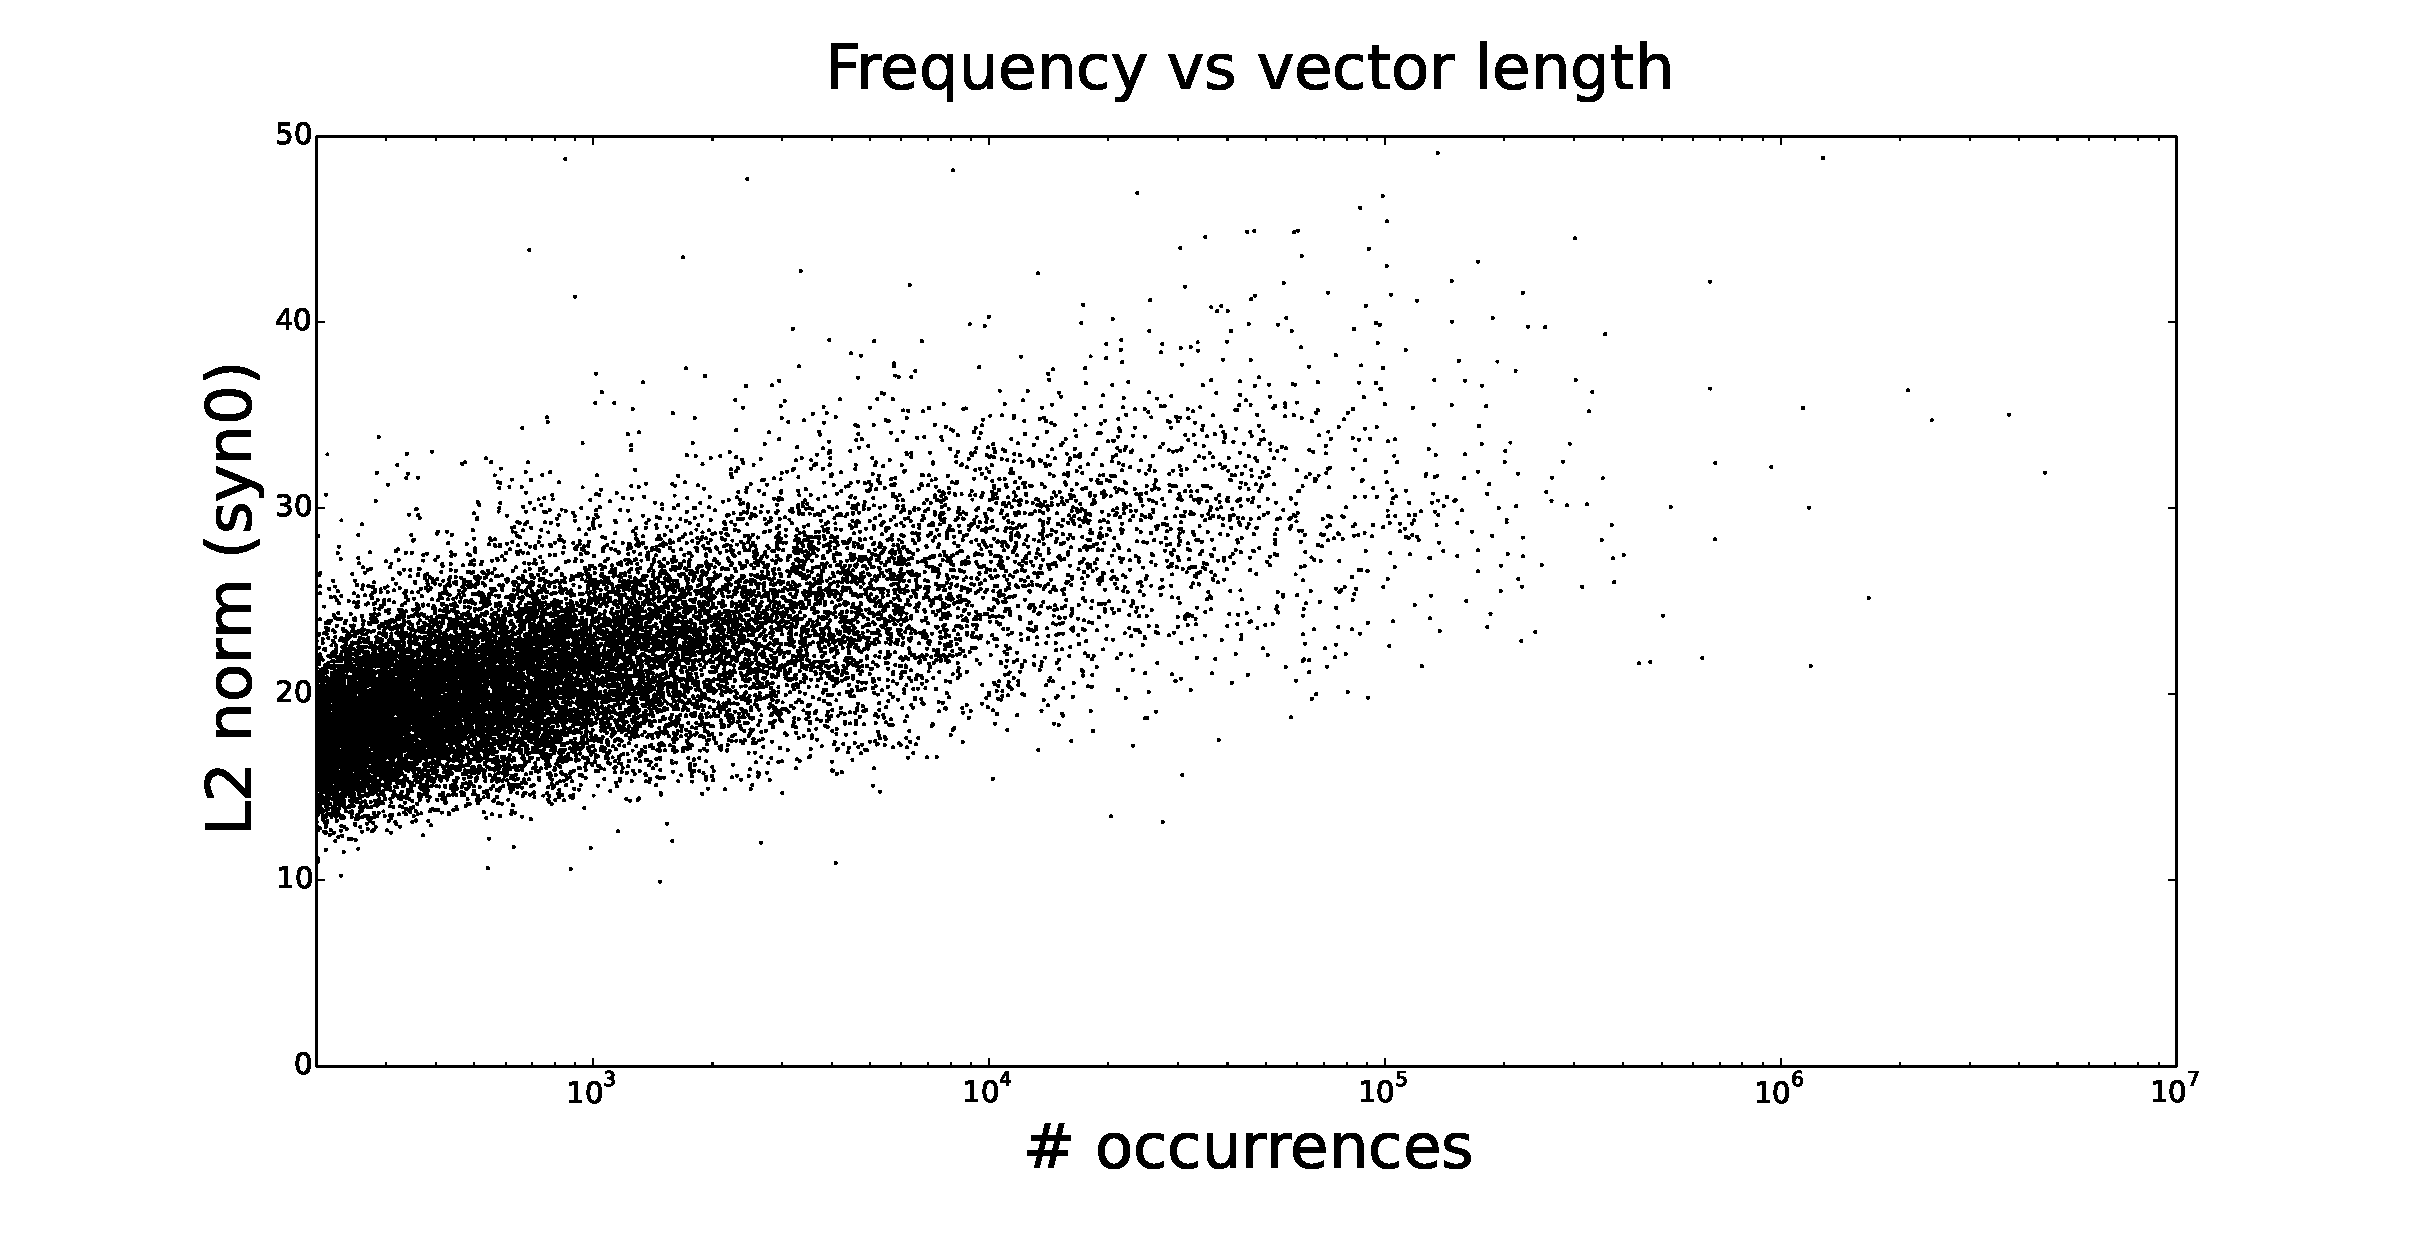
\includegraphics[scale=0.3]{frequency-norm-scatterplot}
	\caption{ The global relationship between word frequency and vector length.  }
	\label{fig:frequency-norm-graph}
\end{figure}

\begin{figure}\label{word-frequency-experiment-heatmap}
	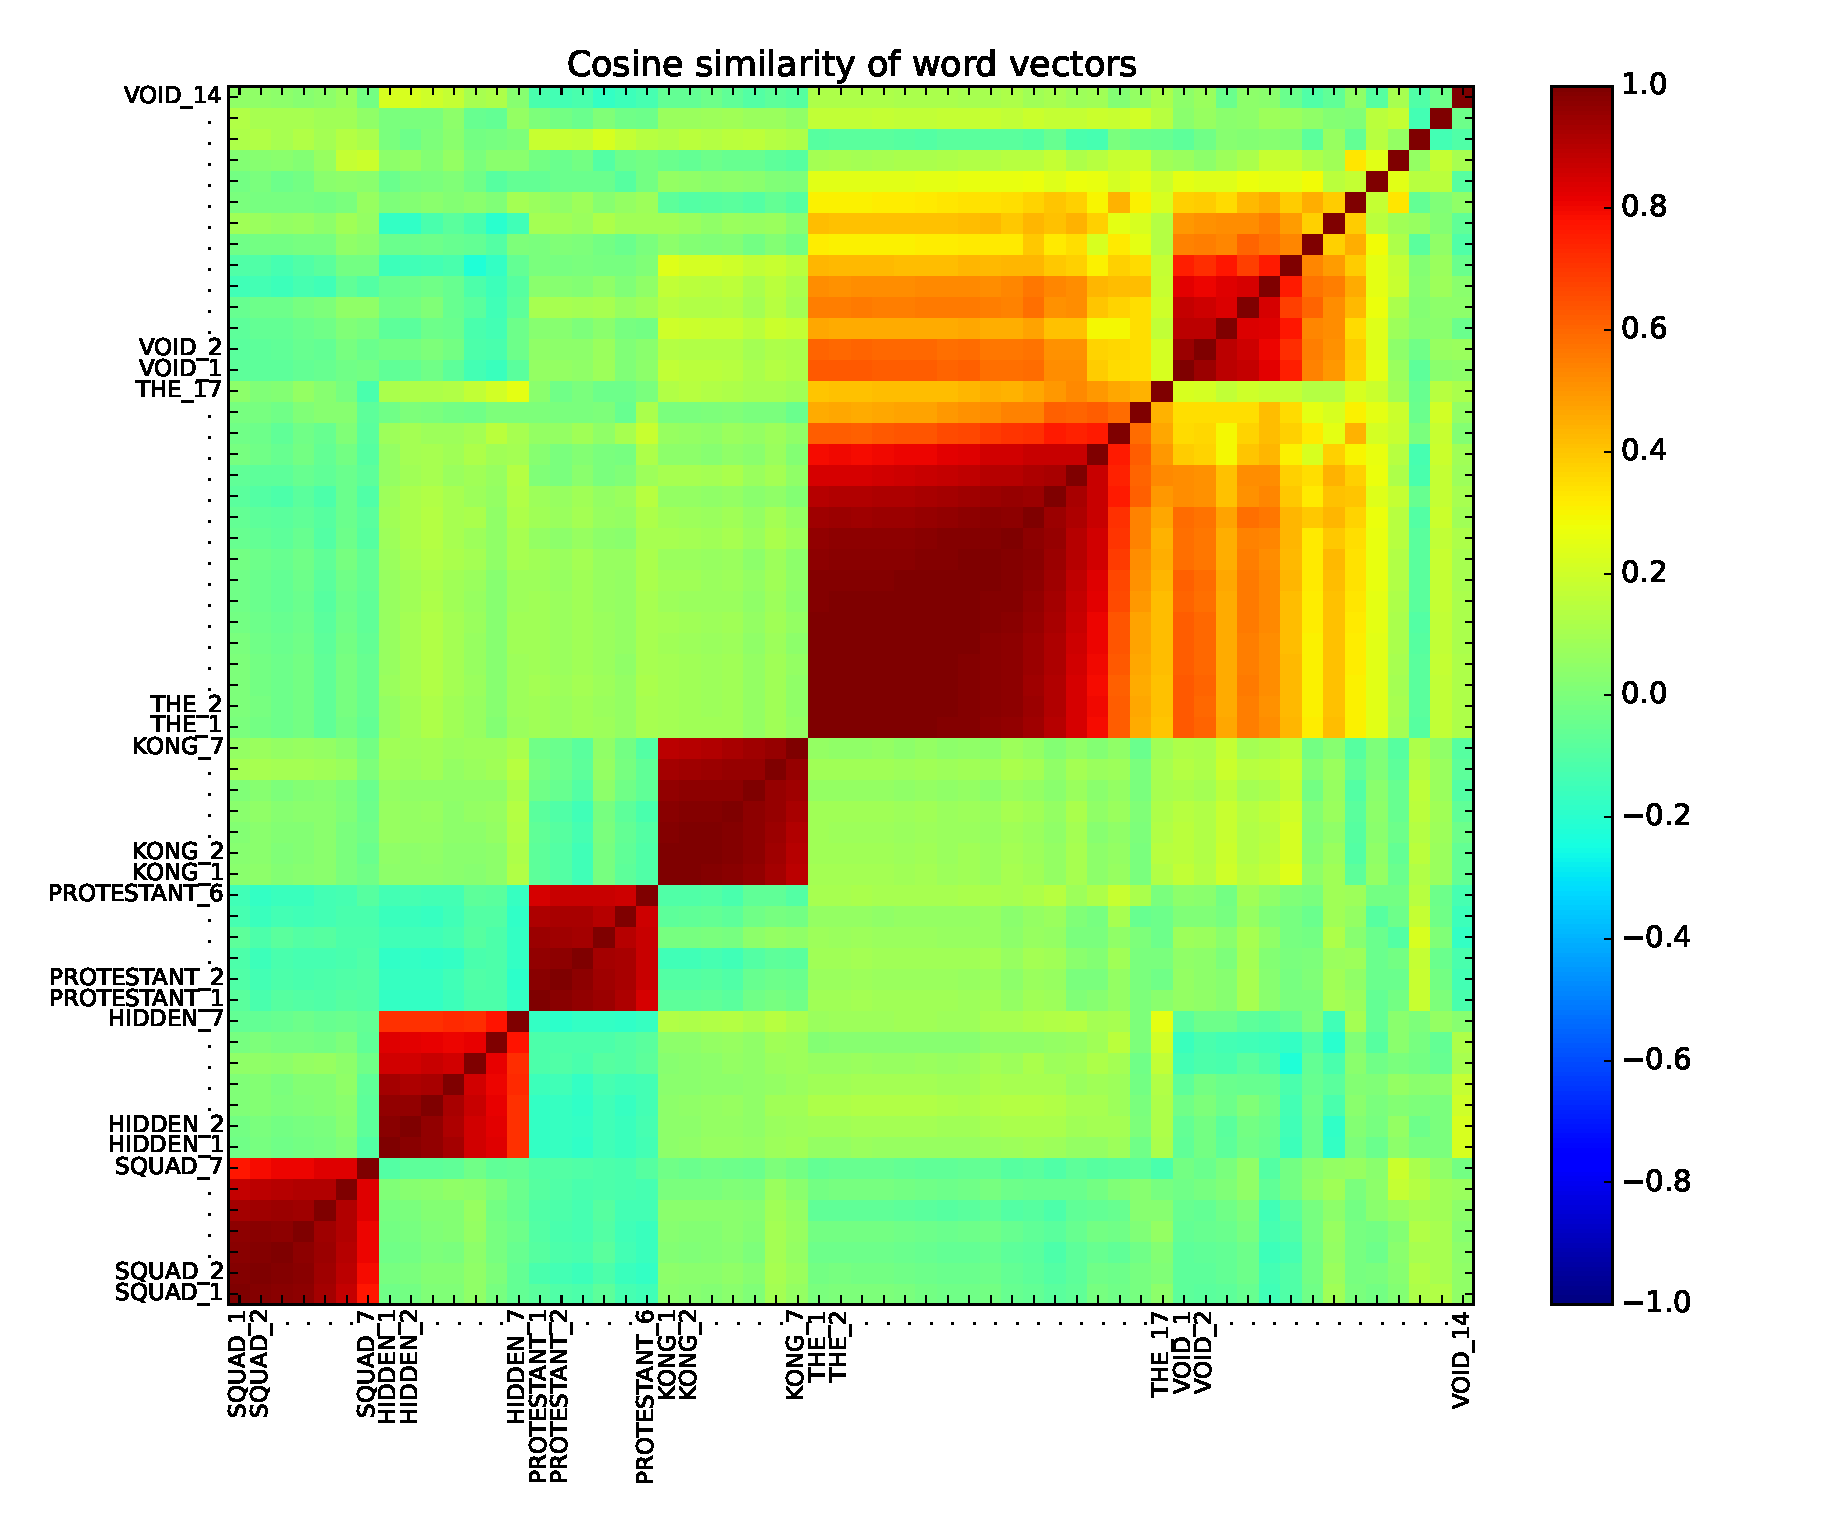
\includegraphics[scale=0.5]{word-frequency-experiment-heatmap}
	\caption{
	Heatmap of the cosine similarity of the vectors associated to the
	tokens introduced into the corpus in the co-occurrence noise experiment
	(words other than \word{the} and \word{VOID} chosen randomly).
	}
\end{figure}

\begin{sidewaysfigure*}\label{fig:word-frequency-experiment-graph}
	\centering{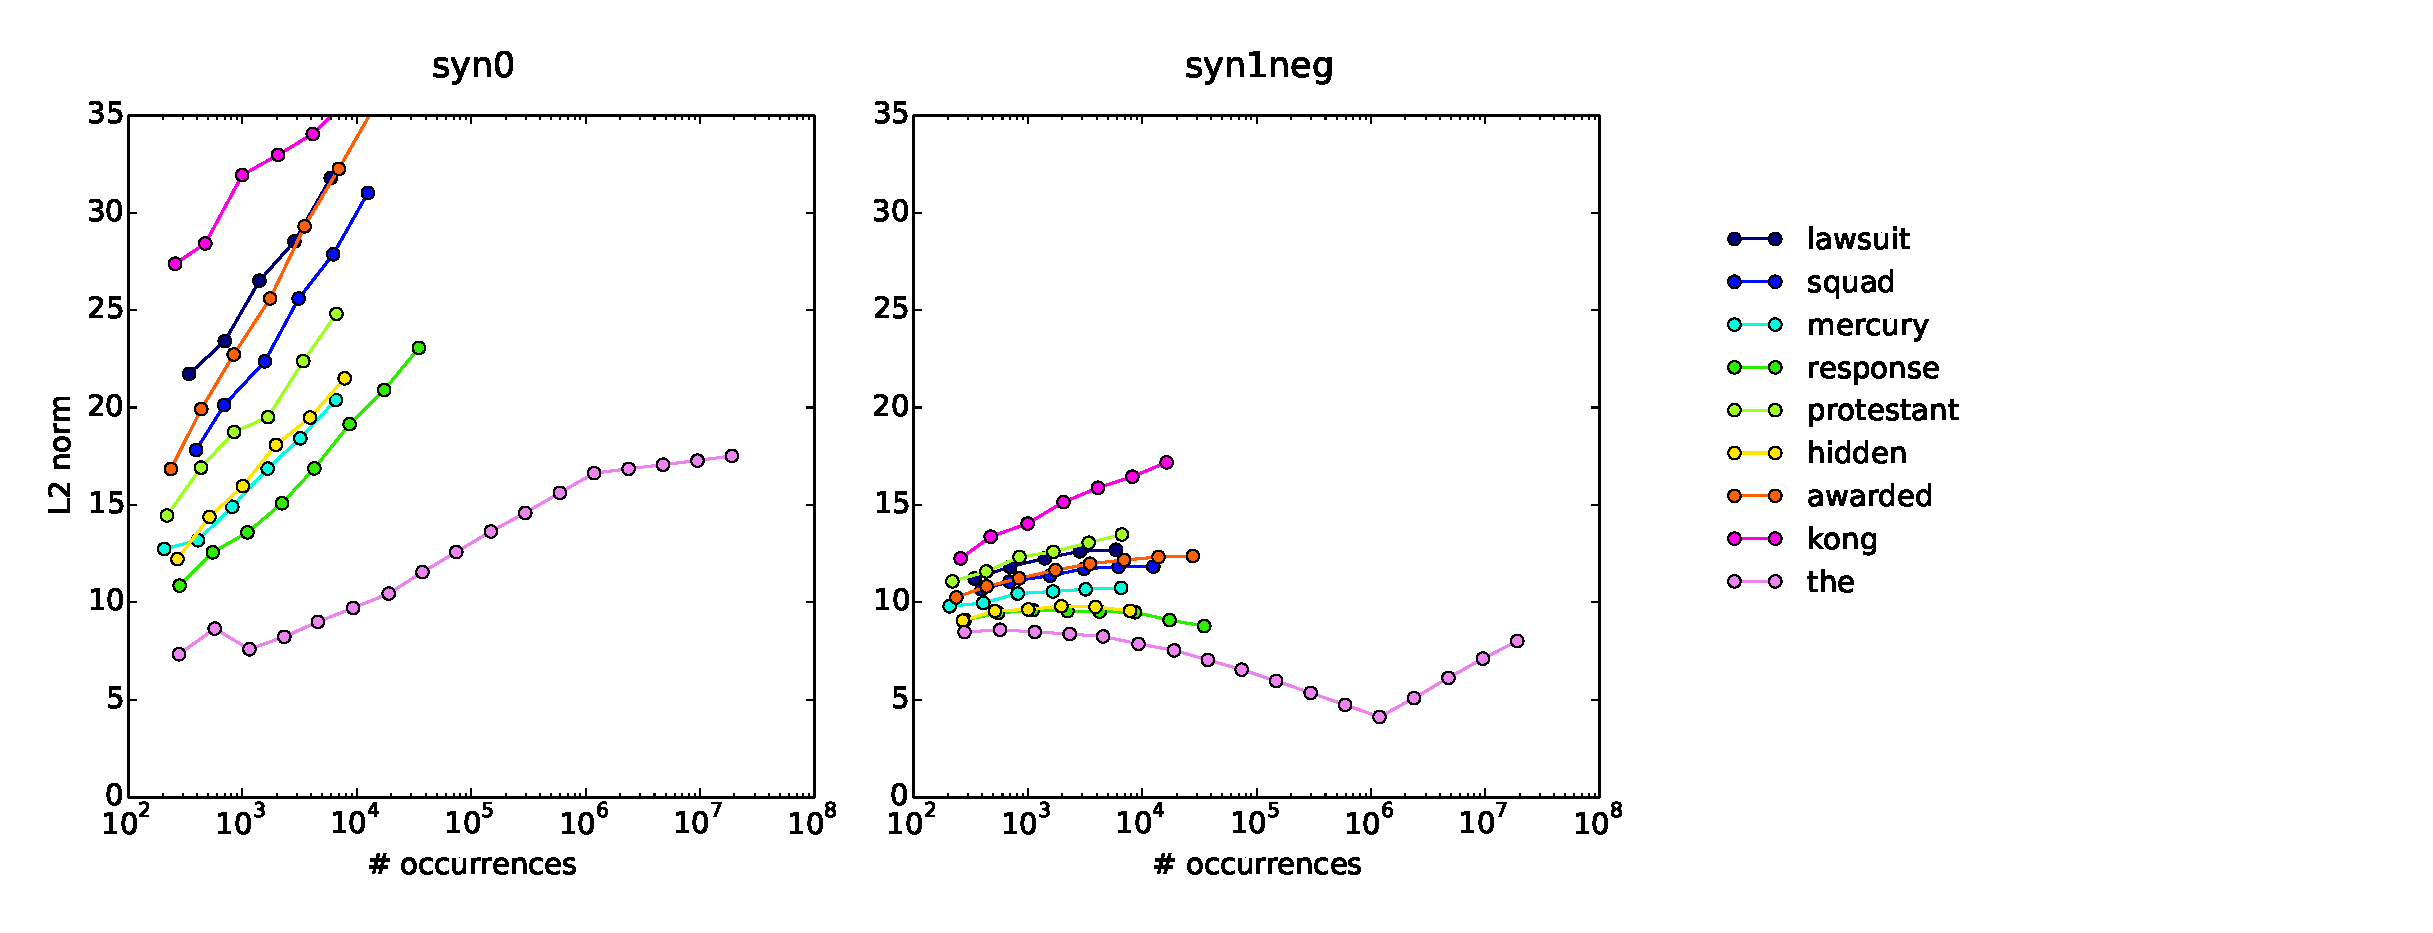
\includegraphics[scale=0.6]{word-frequency-experiment-graph}}
	\caption{
	Vector length vs. frequency for the words chosen for the word frequency
	experiment.  For each word, tokens of varying frequency but with the
	co-occurrence distribution of that word were introduced into the
	corpus, as described in section \ref{WFVE}.
	The word vectors are obtained from the first synaptic layer, ``syn0''.
	The second layer ``syn1neg'' is included for completeness.
	}
\end{sidewaysfigure*}

\end{section}

\begin{section}{Co-occurrence noise variation experiment}\label{CNVE}
Here, and throughout, the noise distribution is taken to be the global word frequency distribution.
Thus noise can be added to the co-occurrence distribution of a word by inspersing occurrences of that word uniformly at randomly throughout the corpus.
A small set of words is chosen from the unmodified corpus in the same manner as in section \ref{WFVE}.

For each of the chosen words, the replacement procedure of subsection \ref{replacement-procedure} is performed using a geometric rate of decay of $\lambda = 5/6$, and truncating at $n=8$.
Subsequently, for every replacement token (e.g. \word{CAT\_i}) random occurrences of this token are interspersed uniformly at random throughout the corpus, such that the frequency of the replacement token is restored to that of the original token \word{cat}.
For example, if the original token \word{cat} occurred $1000$ times, then after the replacement procedure, \word{CAT\_2} occurs approximately $694$ times, so a further (approximately) $306$ random occurrences of \word{CAT\_2} are interspersed throughout the corpus.
Thus token \word{cat} is removed from the corpus, and a family of tokens \word{CAT\_i}, $1 \leqslant i \leqslant 8$ are introduced.
These tokens all have the same frequency as \word{cat}, but their co-occurrence distributions, while based on that of \word{cat}, have an increasing amount of noise.

Figure \ref{fig:co-occurrence-noise-experiment-text} illustrates the effect of this modification, in the case where the only word chosen is \word{cat}.
The original text in this case concerned both cats and dogs.
Notice that the word \word{cat} has been replaced entirely in the cats section by occurrences of \word{CAT\_i} and moreover that occurrences of these same tokens appear also in the dogs section. These occurrences (and additionally, with probability, some occurrences from the cats section) are ``noise occurrences''.

The proportion of the occurrences of \word{CAT\_i} that arose by replacing \word{cat} is $P_{5/6}(i)$, and the proportion arising from the random intersperal of this token throughout the corpus is $r_i := (1 - P_{5/6}(i))$.
The particular value of $\lambda$ (large compared to that of section \ref{WFVE}) was chosen so that the proportion of noise $r_i$ did not increase too quickly with $i$.
These proportions are the sampling points on our axis of variation, and this value of $\lambda$ (together with the choise of $n$) ensures a reasonable spread.
Note that other parameter values (or indeed other distributions) could equally have been used.

\begin{figure}
	\begin{center}
\begin{tabular}{l | r}
word & \# occurrences \\
\hline
\word{dying} & 10693 \\
\word{bridges} & 12193 \\
\word{appointment} & 12546 \\
\word{aids} & 13487 \\
\word{boss} & 14105 \\
\word{removal} & 15505 \\
\word{jobs} & 21065 \\
\word{community} & 115802 \\
\end{tabular}
\end{center}

	\label{fig:co-occurrence-noise-counts}
	\caption{Occurrence counts for words chosen for the co-occurrence noise experiment. }
\end{figure}

\begin{figure}
	\texttt{the domestic \textcolor{red}{CAT\_2} was first classified as felis catus\newline the semiferal \textcolor{red}{CAT\_3} a mostly outdoor \textcolor{red}{CAT\_4} is not \textcolor{red}{CAT\_2} owned by any one individual\newline a pedigreed \textcolor{red}{CAT\_4} is one whose ancestry is recorded by a \textcolor{red}{CAT\_1} fancier organization\newline \textcolor{red}{CAT\_6} a purebred \textcolor{red}{CAT\_3} is one whose ancestry contains only individuals of the same breed\newline the \textcolor{red}{CAT\_1} skull is unusual among mammals in having very \textcolor{red}{CAT\_4} large eye sockets\newline another unusual feature is that the \textcolor{red}{CAT\_4} cannot produce taurine\newline within groups one \textcolor{red}{CAT\_2} is usually dominant over the others\newline ...\newline the domestic dog canis lupus familiaris is a domesticated canid which has been selectively \textcolor{red}{CAT\_5} bred\newline dogs perform many roles for people such as hunting herding and pulling loads\newline \textcolor{red}{CAT\_7} in domestic dogs sexual maturity begins to happen around age six to twelve months\newline this is \textcolor{red}{CAT\_6} the time at \textcolor{red}{CAT\_3} which female dogs will have their first estrous cycle\newline some dog breeds have acquired traits through selective breeding that interfere with reproduction}
	\caption{A text modified for the co-occurrence noise experiment, where the word \word{cat} was chosen, $\lambda = 5/6$ and $n=3$.}
\label{fig:co-occurrence-noise-experiment-text}
\end{figure}

\begin{subsection}{Results}
Figure \ref{fig:co-occurrence-noise-heatmap} shows the cosine similarity of the pairs of word vectors for the tokens introduced into the corpus.
Notice that the word vectors associated to tokens derived from the same word all share a common direction.
We conclude that co-occurrence noise has no effect on word vector direction.

On the other hand, Figure \ref{fig:co-occurrence-noise-graph} shows that word vector length varies directly and linearly with the proportion $r$ of noise in the co-occurrence distribution.
This figure motivates an interpretation of vector length, within a sufficiently narrow frequency band, as a measure of the absence of co-occurrence noise, that is, of the extent to which a word determines a context.


\begin{figure}\label{fig:co-occurrence-noise-heatmap}
	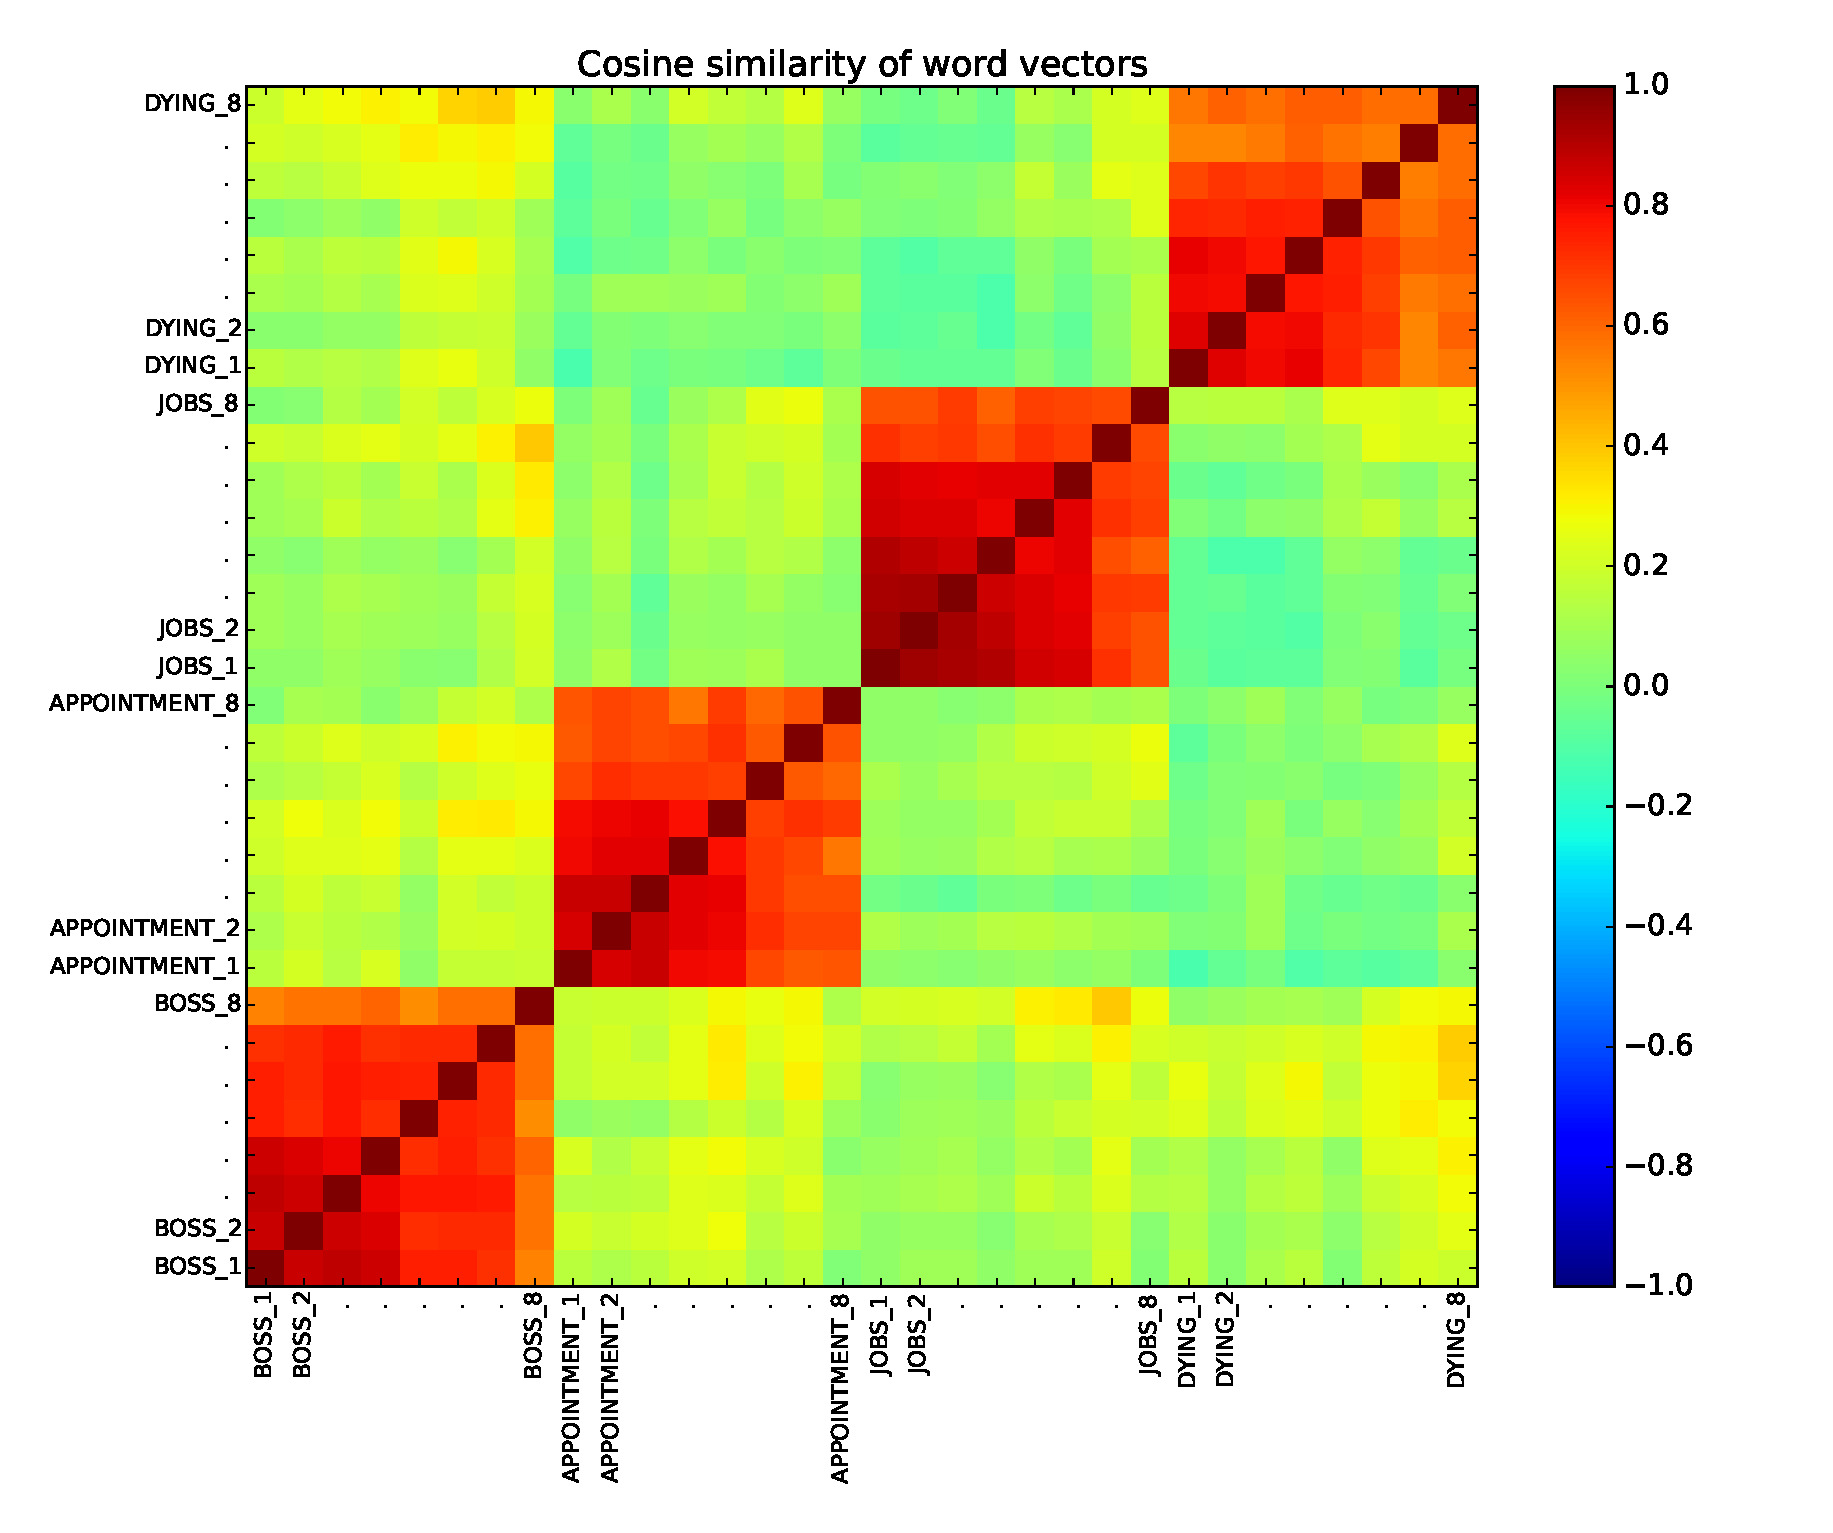
\includegraphics[scale=0.5]{cooccurrence-noise-heatmap}
	\caption{
	Heatmap of the cosine similarity of some of the vectors associated to the
	tokens introduced into the corpus in the co-occurrence noise experiment
	(four such words chosen at random).  The
	largely red blocks demonstrate that the direction of the word vector
	does not change when noise is added to the co-occurrence distribution.
	}
\end{figure}

\begin{sidewaysfigure*}\label{fig:co-occurrence-noise-graph}
	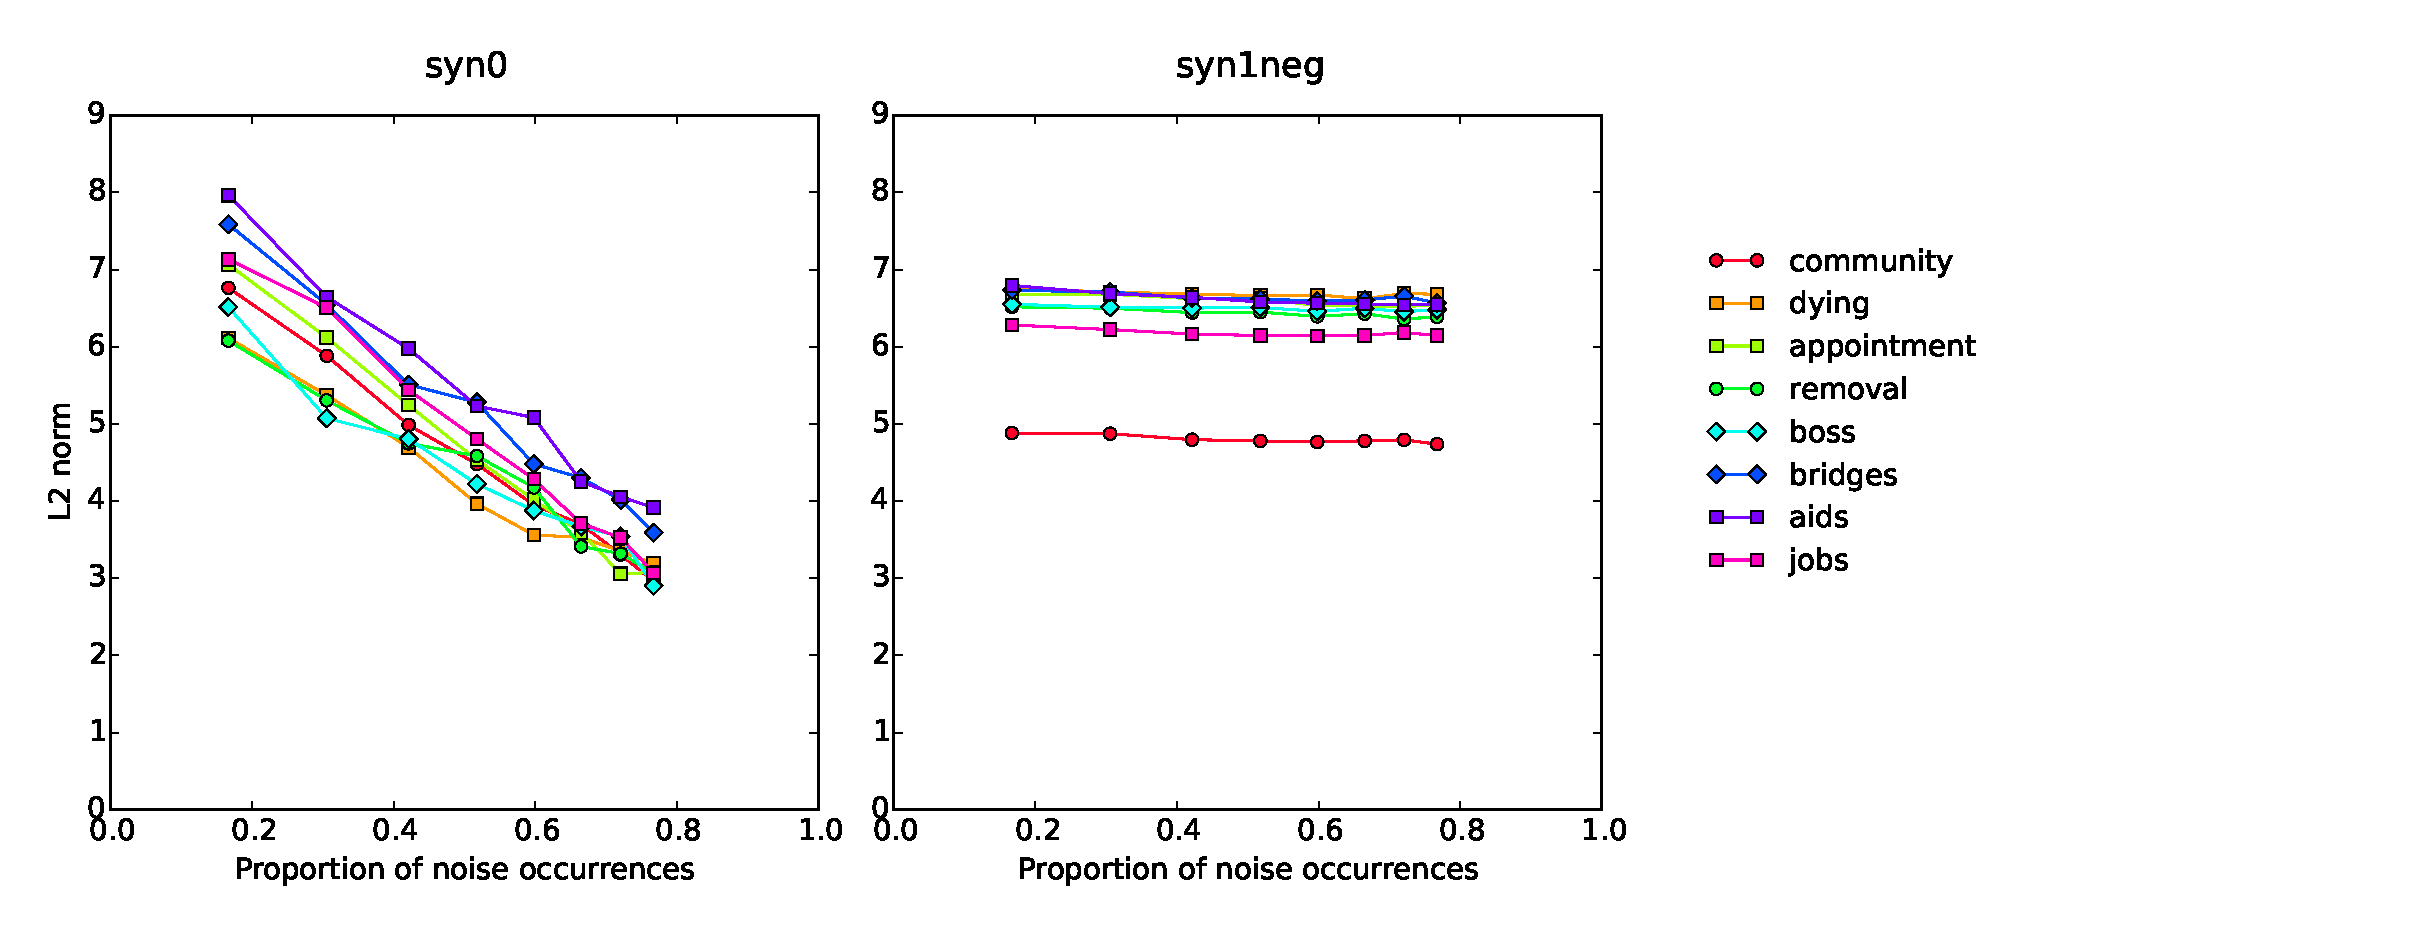
\includegraphics[scale=0.6]{cooccurrence-noise-graph}
	\caption{
	Vector length vs. proportion of co-occurrence noise for words
	chosen for the co-occurrence noise experiment.  For each word,
	tokens of equal frequency but with increasing proportions of
	co-occurrence noise were introduced into the corpus, as
	described in section \ref{CNVE}.
	The word vectors are obtained from the first synaptic layer, ``syn0''.
	The second layer ``syn1neg'' is included for completeness.
	}
\end{sidewaysfigure*}

\end{subsection}

\end{section}

\begin{section}{Discussion and future directions}\label{future-directions}

\begin{subsection}{Controlled experiments for word embeddings}
The principle contribution of this short note has been to demonstrate that controlled experiments can be used to gain insight into any word embedding.
Because they are achieved via modification of the training corpus, these experiments can be carried out for any language model or word embedding.
The experiments are moreover easy to carry out, requiring modification of code nor even knowledge of the model itself.

More elaborate experiments could be carried out in the context of word embeddings.
For instance, by introducing tokens into the corpus that mix, with varying proportions, the co-occurrence distributions of two words, the path between the word vectors in the feature space can be studied.
The co-occurrence noise variation experiment described here would be a special case of such an experiment where one of the two words was \word{VOID}.

It would, of course, be interesting to perform these experiments for other word embeddings and for different hyperparameters settings.
\end{subsection}

\begin{subsection}{Applications in other contexts}
Further afield, it would be interesting to perform analogs of these experiments in other contexts where models are trained from co-occurrence data.
For instance, in the context of e-Commerce, product purchase frequency and product co-occurrence noise can be varied by modifying the item-item matrix.
\end{subsection}

\begin{subsection}{Questions pertaining to word2vec}
Questions pertaining to particularly to word2vec arise naturally from the results of the experiments.
Figures \ref{fig:frequency-norm-graph} and \ref{fig:co-occurrence-noise-graph}, for example, demonstrate the word vectors obtained from the first synaptic layer, ``syn0'', have very different properties from those that could be obtained from the second layer, ``syn1neg'', which are typically discarded.
These differences warrant further investigation.

The co-occurrence distribution of \word{VOID} is the global frequency distribution, and in this sense pure background noise.
Thus the word vector of \word{VOID} is a special point in the feature space.
Figure \ref{fig:frequency-norm-graph} shows that this point is not at the origin of the feature space (i.e. is not the zero vector).
It is the origin, however, that is implicitly used as the point of reference in the word2vec word similarity task.
This raises the question of whether improved performance on the similarity task could be achieved by transforming the feature space (or modifying the model) such that the representation of pure noise (i.e. the vector for \word{VOID}) was at the origin of the transformed feature space. 
\end{subsection}

\end{section}

\clearpage
\footnotesize
\bibliography{main}
\bibliographystyle{plain}
\end{document}
